\documentclass[a4paper]{article}
\usepackage[UTF8]{ctex}
\usepackage{geometry}
\usepackage{graphicx}
\usepackage{url}
\usepackage{multirow}
\usepackage{array}
\usepackage{booktabs}
\usepackage{url}
\usepackage{enumitem}
\usepackage{graphicx}
\usepackage{float}
\usepackage{amssymb}
\usepackage{amsmath}
\usepackage{subfig}
\usepackage{longtable}
\usepackage{pifont}
\usepackage{color}
\usepackage{listings}
\usepackage{xcolor}

\allowdisplaybreaks

\geometry{a4paper, scale=0.78}

% \begin{figure}[H]
%     \centering
%     \includegraphics[width=.55\textwidth]{E.png}
%     \caption{矩阵与列向量的乘法}
%     \label{fig:my_label_1}
% \end{figure}

% \left\{
% \begin{array}{ll}
%       x+2x+z=2 & \\
%       3x+8y+z=12 & \\
%       4y+z=2
% \end{array}
% \right.

% \begin{enumerate}[itemindent = 1em, itemsep = 0.4pt, parsep=0.5pt, topsep = 0.5pt]

% \end{enumerate}

%\stackrel{a}{\longrightarrow}

\title{Probability Graph 04 Example}
\author{Chen Gong}
\date{26 November 2019}

\begin{document}
\maketitle
上一节中,我们讲的是模型通用的一些概念,这一节开始,我们要讲一讲贝叶斯网络具体的例子。我们从单一,混合,时间和连续,四个角度来看看Bayesian Network,这个四个方法是一步一步越来越难的。

\section{单一}
单一最典型的代表就是Naive Bayesian,这是一种classification的模型。对于$p(x|y)$的问题来说,假设各维度之间相互独立,于是就有:
\begin{equation}
    p(x|y) = \prod_{i=1}^N p(x_i|y=1)
\end{equation}

概率图模型表示如下所示:
\begin{figure}[H]
    \centering
    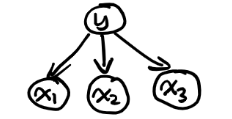
\includegraphics[width=.35\textwidth]{微信图片_20191125225919.png}
    \caption{Naive Bayesian Network拓扑表示}
    \label{fig:my_label_1}
\end{figure}

很显然是一个Tail to Tail的模型,我们很简单可以得出$x_1 \bot x_2 \bot \cdots \bot x_N$。

\section{混合}
最常见的就是Gaussian Mixture Model (GMM),这是一种聚类模型,将每个类别拟合一个分布,计算数据点和分布之间的关系来确定,数据点所属的类别。我们假设$Z$是一个隐变量,并且$Z$是离散的变量,那么$x|z \sim \mathcal{N}(\mu,\Sigma)$。我们用模型可以表示为:
\begin{figure}[H]
    \centering
    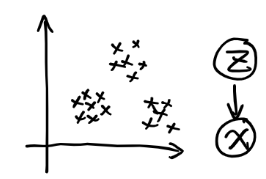
\includegraphics[width=.35\textwidth]{微信图片_20191125231235.png}
    \caption{Gaussian Mixture Model的可视化表示}
    \label{fig:my_label_1}
\end{figure}

\section{时间}
时间上我们大致可以分成两种。第一种是Markov chain,这是随机过程中的一种;第二种事Gaussian Processing,实际上就是无限维的高斯分布。

实际上时间和混合可以一起看,我们称之为动态系统模型。并且,我们就可以衍生出三种常见的模型,这里讲的比较的模糊,在后面的章节我们会进行详细的分析。第一种是隐马尔可夫模型(HMM),这是一种离散的模型;第二种是线性动态系统(LDS),这是一种线性的连续的模型,包括典型的Kalman Filter。第三种是Particle Filter,一种非高斯的,非线性的模型。

\section{连续}
连续就是Guassian Bayesian Network,前面有提到过。

~\\

大家可能听到这么多的名词会一脸懵逼呀,懵逼是很正常的,因为这些名词只是给了个印象,后面我们会进行详细的分析。实际上一个整体的趋势就是{\color{red} 从单一到混合,从有限到无限。}也就是从空间和时间两个角度来进行分析,都是从离散到连续的过程。至于具体为什么这么分,还得具体学习了算法我们才能够很好的理解,本小节只是起了一个高屋建瓴的作用。




















\end{document}
